\documentclass{beamer}

\mode<presentation> {
	
	% The Beamer class comes with a number of default slide themes
	% which change the colors and layouts of slides. Below this is a list
	% of all the themes, uncomment each in turn to see what they look like.
	
	%\usetheme{default}
	%\usetheme{AnnArbor}
	%\usetheme{Antibes}
	%\usetheme{Bergen}
	%\usetheme{Berkeley}
	%\usetheme{Berlin}
	%%%\usetheme{Boadilla}
	%\usetheme{CambridgeUS}
	%\usetheme{Copenhagen}
	%%%\usetheme{Darmstadt}
	%%%\usetheme{Dresden}
	\usetheme{Frankfurt}
	%\usetheme{Goettingen}
	%\usetheme{Hannover}
	%\usetheme{Ilmenau}
	%\usetheme{JuanLesPins}
	%\usetheme{Luebeck}
	%\usetheme{Madrid}
	%\usetheme{Malmoe}
	%%%\usetheme{Marburg}
	%%%\usetheme{Montpellier}
	%\usetheme{PaloAlto}
	%\usetheme{Pittsburgh}
	%\usetheme{Rochester}
	%\usetheme{Singapore}
	%\usetheme{Szeged}
	%\usetheme{Warsaw}
	
	% As well as themes, the Beamer class has a number of color themes
	% for any slide theme. Uncomment each of these in turn to see how it
	% changes the colors of your current slide theme.
	
	%\usecolortheme{albatross}
	%%%\usecolortheme{beaver}
	%\usecolortheme{beetle}
	%\usecolortheme{crane}
	%\usecolortheme{dolphin}
	%\usecolortheme{dove}
	%\usecolortheme{fly}
	%\usecolortheme{lily}
	%\usecolortheme{orchid}
	%\usecolortheme{rose}
	%\usecolortheme{seagull}
	%\usecolortheme{seahorse}
	%\usecolortheme{whale}
	%\usecolortheme{wolverine}
	
	%\setbeamertemplate{footline} % To remove the footer line in all slides uncomment this line
	\setbeamertemplate{footline}[page number] % To replace the footer line in all slides with a simple slide count uncomment this line
	
	\setbeamertemplate{navigation symbols}{} % To remove the navigation symbols from the bottom of all slides uncomment this line
}


\usepackage[utf8]{inputenc}
\usepackage[ukrainian]{babel}

\usepackage{amssymb}
\usepackage{physics}


\usepackage[active]{srcltx}
\usepackage[final]{pdfpages}

\usepackage{verbatim}

\usepackage{graphicx} % Allows including images
\usepackage{booktabs} % Allows the use of \toprule, \midrule and \bottomrule in tables

\numberwithin{equation}{section}

%------------------------------------------------

 \newcommand{\tabboxl}[2]{\parbox{#1}{\vspace{0.1cm} #2 \vspace{0.1cm} }}

\newcommand{\tabboxr}[2]{\parbox{#1}{\vspace{-0.3cm}
		\begin{flushright} #2 \end{flushright} \vspace{-0.3cm} }}

\newcommand{\tabboxc}[2]{\parbox{#1}{\vspace{-0.3cm}
		\begin{center} #2 \end{center} \vspace{-0.3cm} }}

\newcommand{\liml}{\lim\limits}
\newcommand{\suml}{\sum\limits}
\newcommand{\intl}{\int\limits}

\newcommand{\inttwopi}{\intl_{0}^{2\pi}}

\newcommand{\boundprob}{(\ref{laplace-eq}) -- (\ref{neumann-condition})}

\newtheorem{thm}{\protect\thmname}
\renewcommand{\thmname}{Теорема}

%----------------------------------------------------------------------------------------
%	TITLE PAGE
%----------------------------------------------------------------------------------------


\title[Short title]{Розробка алгоритмів захисту від атак на глибокі нейронні мережі} % The short title appears at the bottom of every slide, the full title is only on the title page

\author{Бугрій Богдан} % Your name
\institute[UCLA] % Your institution as it will appear on the bottom of every slide, may be shorthand to save space
{
	Львівський національний університет імені Івана Франка \\
	Факультет прикладної математики та інформатики 
}
\date{\today} % Date, can be changed to a custom date

\begin{document}
	%------------------------------------------------
	
	\begin{frame}
		\titlepage
	\end{frame}
	
	%------------------------------------------------
	
	\begin{frame}
		\frametitle{План}
		\tableofcontents
	\end{frame}

	%------------------------------------------------
	\section{Опис проблеми}
	%------------------------------------------------
	
	%\subsection{Постановка задачі}

	\begin{frame}
		\frametitle{Проблема}
		Нехай $M$ -- система машинного навчання, $x\in \mathbb{R}^n$ -- вхідний зразок, $y_{true}\in \mathbb{R}^C$ - правильне передбачення для зразка $x$, тобто 
		\begin{equation}
			M(x) = y_{true}
		\end{equation} 
		Можна створити зразок $x^{adv}=x+\tau$, де $\tau\in \mathbb{R}^n$, такий, що 
		\begin{equation}
			M(x^{adv})\neq y_{true}
		\end{equation}
	\end{frame}

	\begin{frame}
		\frametitle{Постановка задачі}
		Нехай $S^{adv}(M) \subset S$ -- множина ошукуючих зразків для моделі $M$. Необхідно знайти модель $M'$ таку, що
		\begin{equation}
			S^{adv}(M') = \emptyset.
		\end{equation}
		%Мається на увазі, що для моделі $M'$ неможливо створити ошукуючі зразки, тобто вона є невразливою до атак. 
		%Такий ``ідеальний'' випадок є практично неможливим, тому ми будемо використовувати пом'якшене формулювання, а саме вимагатимемо, щоб для моделі-образа задовільнялася умова
		На практиці модель-образа повинна задовільняти умову
		\begin{equation}
			n(S^{adv}(M')) < n(S^{adv}(M))
		\end{equation}
		де $n(S)$ --кількість елементів в множині $S$.
		% Іншими словами, нашою метою є побудова моделі, більш стійкої до атак, ніж оригінал.
	\end{frame}


	%-------------------------------------------------
	%\subsection{Типи захисту}
	\begin{frame}
		\frametitle{Типи захисту}
		\begin{block} {За типом атак} 
			\begin{itemize}
				\item Захист від ошукуючих атак.
				\item Захист від викрадення.
				\item Захист від отруєння.
			\end{itemize}
		\end{block}
		\vspace{.5cm}
		\begin{block} {За стратегією захисту}
			\begin{itemize}
				\item Модифікація архітектури моделі та процесу тренування.
				\item Генерація специфічного тренувального набору.
				\item Створення захисної оболонки.
			\end{itemize}
		\end{block}	
	\end{frame}
	\begin{comment}
	\begin{columns}
	\begin{column}{.40\textwidth}
	\begin{block} {За типом атак} 
	\begin{itemize}
	\item захист від ошукуючих атак.
	\item захист від викрадення.
	\item захист від отруєння.
	\end{itemize}
	\end{block}	
	\end{column}
	\begin{column}{.40\textwidth}
	\begin{block} {За стратегією захисту}
	\begin{itemize}
	\item Модифікація архітектури моделі та процесу тренування.
	\item Генерація специфічного тренувального набору.
	\item Створення захисної оболонки.
	\end{itemize}
	\vspace{.85cm}
	\end{block}	
	\end{column}
	\end{columns}
	\end{comment}
	
	%------------------------------------------------
	\section{Ошукуючі зразки}
	%------------------------------------------------
	%\subsection{Природа ошукуючих зразків}
	\begin{frame}
		\frametitle{Природа ошукуючих зразків}
		\begin{figure}[h]
			\centering
			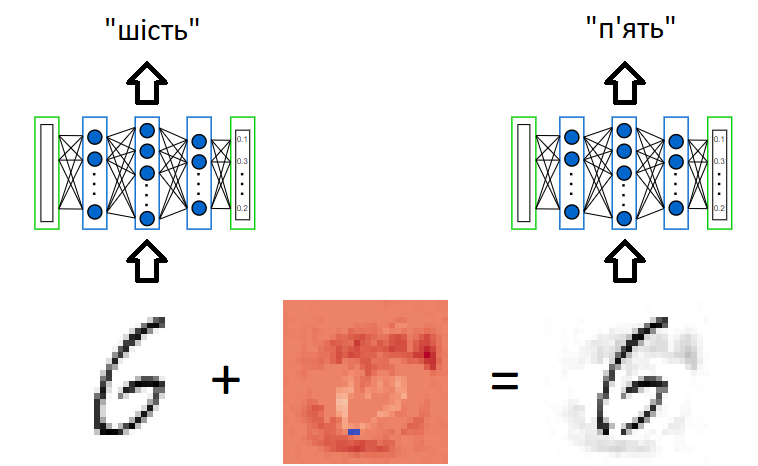
\includegraphics[width=.9\textwidth]{../images/six-p.png}
			
			%\caption{Область $D$}
			%\label{fig:double-connected-region}
		\end{figure}
	\end{frame}
	
	\begin{comment}
	\subsection{}
	\begin{frame}
		\frametitle{Атаки}
		
	\end{frame}
	\end{comment}


	%------------------------------------------------
	\section{Стійкість}
	%\subsection{}
	\begin{frame}
		\frametitle{Стійкість}
		
		\begin{figure}[h]
			\centering
			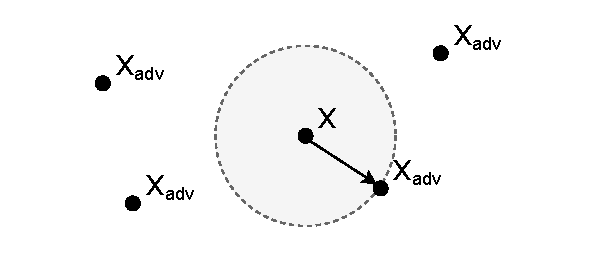
\includegraphics[width=0. 8\textwidth]{../images/2Dball.pdf}
			
			%\caption{Область $D$}
			%\label{fig:double-connected-region}
		\end{figure}
		%Ідея, на якій базується визначення стійкості:
		\begin{equation}
			\forall \tau \in B_{p}(L): \hat{y}_{k}(x+\tau)>\max _{i: i \neq k} \hat{y}_{i}(x+\tau)
		\end{equation}
		%де $k:=M(x)$, $\hat{y}$ -- вектор ймовірностей.
		
	\end{frame}
	\begin{frame}
		\frametitle{Метрика стійкості}
		\begin{equation}
			\label{robustness-metric}
			r_p(M, X_{test}) := \frac{\sum\limits^{n_{test}}_{i = 1}\|x_i-x^{adv}_i\|_{p}}{n_{test}}
		\end{equation}
	\end{frame}

	\begin{comment}
	\begin{columns}
	\begin{column}{.50\textwidth}
	
	%Метрика для визначення стійкості:
	\begin{equation}
	\label{robustness-metric}
	r_p(M, X_{test}) := \frac{\sum\limits^{n_{test}}_{i = 1}\|x_i-x^{adv}_i\|_{p}}{n_{test}}
	\end{equation}
	%де $n_{test}$ = $n(X_{test})$
	
	\end{column}
	
	\begin{column}{.50\textwidth}
	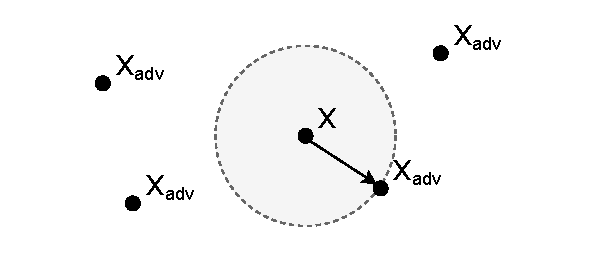
\includegraphics[width=0.45\paperwidth]{../images/2Dball.pdf}
	\end{column}
	\end{columns}
	\end{comment}

	\begin{comment}
	\begin{figure}[h]
	\centering
	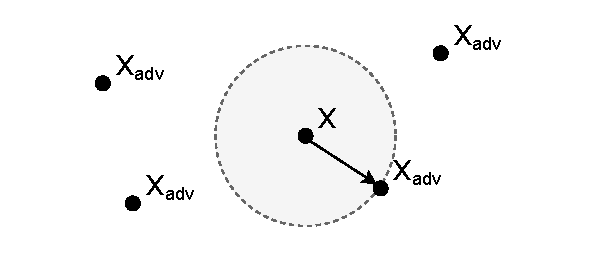
\includegraphics[width=1\textwidth]{../images/2Dball.pdf}
	
	%\caption{Область $D$}
	%\label{fig:double-connected-region}
	\end{figure}
	\end{comment}
	%------------------------------------------------
	
	
	%------------------------------------------------
	\section{Захисна дистиляція}
	%\subsection{Ідея методу}
	\begin{frame}
		\frametitle{Захисна дистиляція}
	
		\begin{figure}[h]
			\centering
			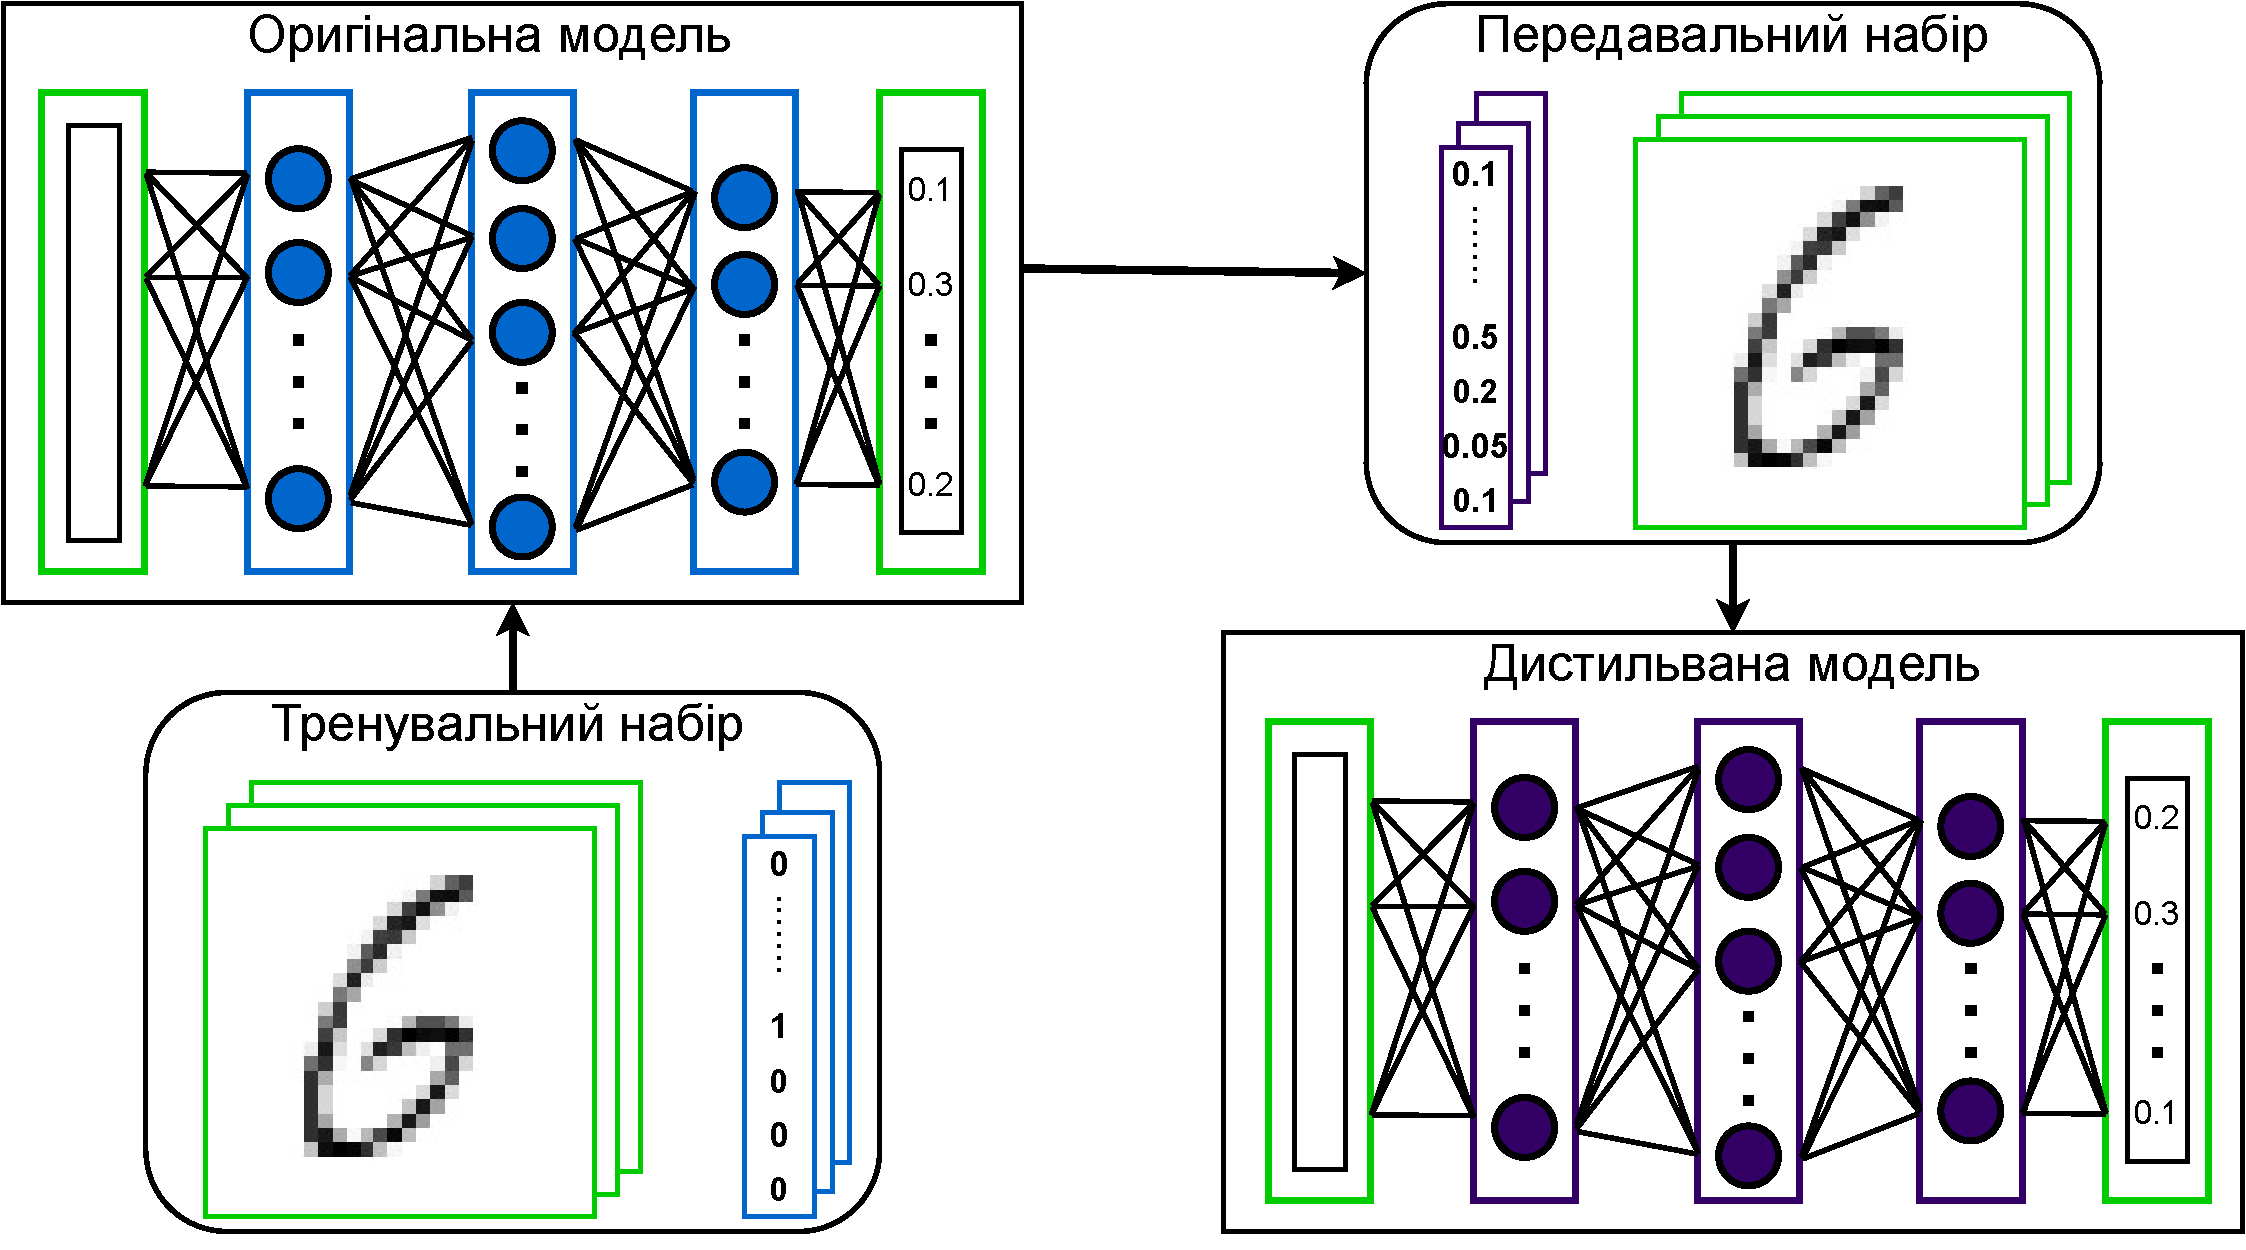
\includegraphics[width=1\textwidth]{../images/diagrams-Distillation.pdf}
			
			%\caption{Область $D$}
			%\label{fig:double-connected-region}
		\end{figure}
	\end{frame}

	%\subsection{Основні параметри}
	\begin{frame}
		\frametitle{Основні параметри}
		
		\begin{equation}
			\label{softmax-t}
			\hat{y}_i(x)=\frac{e^{z_{i}(x) / T}}{\sum\limits_{i=0}^{C-1} e^{z_{i}(x) / T}}, \quad i \in 0 \dots C-1
		\end{equation}
		
		\begin{figure}[h]
			\centering
			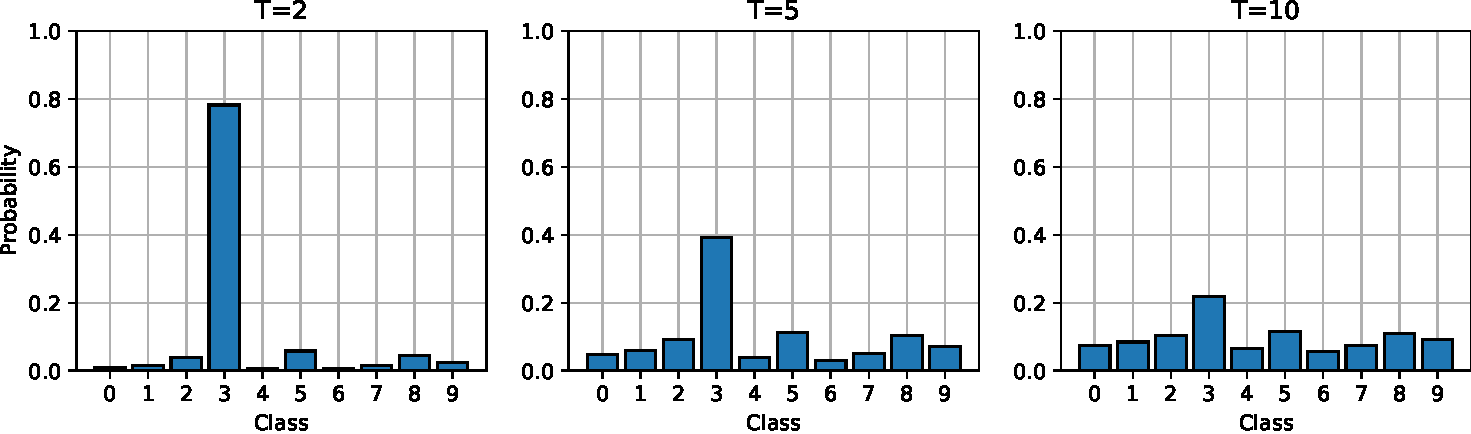
\includegraphics[width=0.8\textwidth]{../images/TvsP.pdf}
			
			\caption{Ймовірності приналежності зразків класу ``трійка'' до інших класів на основі класифікації.}
			%\label{fig:double-connected-region}
		\end{figure}
	\end{frame}


	%\subsection{Переваги та недоліки}	
	\begin{frame}
		\frametitle{Переваги та недоліки}
		\begin{block}{Переваги}
			\begin{itemize}
				\item 
			\end{itemize}
		\end{block}
	
		\begin{block}{Недоліки}
			\begin{itemize}
				\item 
			\end{itemize}
		\end{block}
	\end{frame}
	%------------------------------------------------
	
	
	%------------------------------------------------
	\section{Захист PixelDP}
	%\subsection{}
	\begin{frame}
		\frametitle{Захист PixelDP}
		
		\begin{figure}[h]
			\centering
			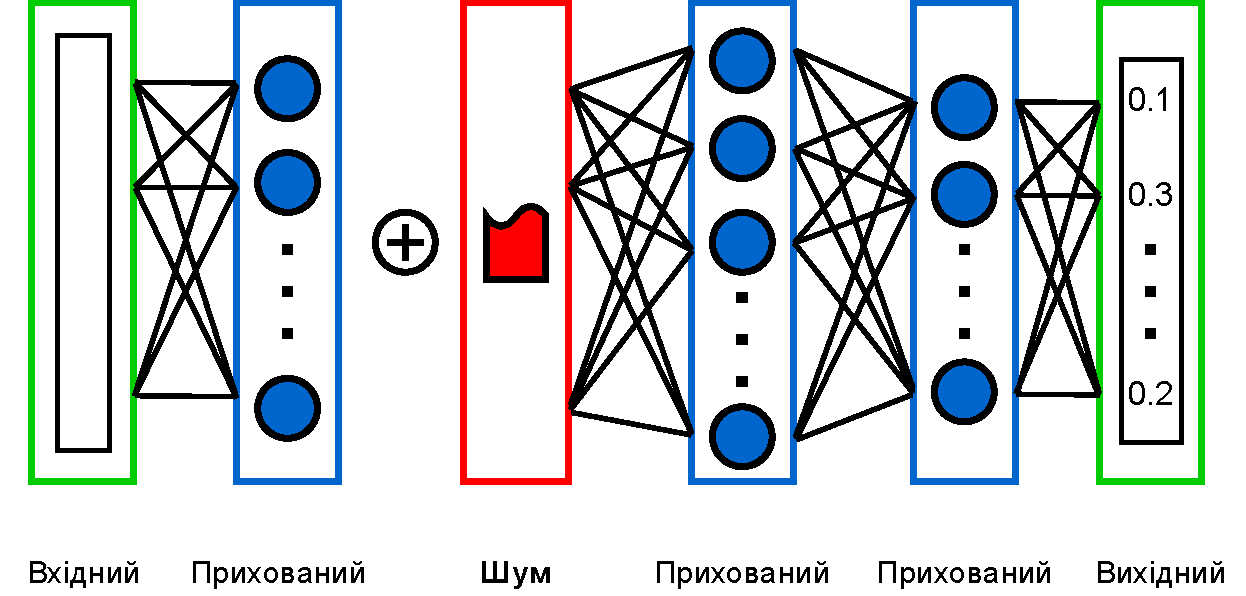
\includegraphics[width=0.9\textwidth]{../images/diagrams-PixelDP-small-p.pdf}
			
			%\caption{Область $D$}
			%\label{fig:double-connected-region}
		\end{figure}
	\end{frame}

	%\subsection{}
	\begin{frame}
		\frametitle{Вимоги до архітектури}
		\begin{block}{Фіксована чутливість}
			 \begin{equation}
				\label{sensitivity}
				\Delta_{p, q}=\Delta_{p, q}^{g}=\max _{x \neq \tilde{x}} \frac{\left\|g(x)-g\left(\tilde{x}\right)\right\|_{q}}{\left\|x-\tilde{x}\right\|_{p}}
			\end{equation}
		\end{block}
	\vspace{0.3cm}
		\begin{block}{Розподіл захисного шуму}
			 \begin{itemize}
				\item \textit{Розподіл Лапласа} при $\mu = 0$ та $\sigma=\sqrt{2} \Delta_{p, 1} L / \epsilon$. 
				\item \textit{Розподіл Гауса} при $\mu = 0$ та $\sigma=\sqrt{2 \ln \left(\frac{1.25}{\delta}\right)} \Delta_{p, 2} L / \epsilon$, $\epsilon \leq 1$
			\end{itemize}
		\end{block}
	\vspace{0.3cm}
		\begin{block}{Очікуване передбачення}
			\begin{equation}
				M_n(x) = argmax\left(\frac{1}{n}\sum\limits_{i = 0}^{n-1}\hat{y}(x)\right)
			\end{equation}
		\end{block}
	    
	\end{frame}

	\subsection{}
	\begin{frame}
		%\frametitle{}
		\begin{block}{Переваги}
			\begin{itemize}
				\item Гарантує стійкість до малих збурень
				\item Зберігає точність моделі прообразу (для великих $n$)
				\item Зловмиснику важко аналізувати ошукуючі градієнти
				\item Невеликі затрати на тренування моделі
			\end{itemize}
		\end{block}
		
		\begin{block}{Недоліки}
			\begin{itemize}
				\item Затратний і неоднозначний процес передбачення
				\item Важко гарантувати стійкість проти великих збурень
			\end{itemize}
		\end{block}
	\end{frame}

	
	%------------------------------------------------
	
	
	%------------------------------------------------
	\section{Експерименти}
	\begin{frame}
		\frametitle{Вплив параметрів на стійкість моделі}
		
		\begin{figure}[h]
			\centering
			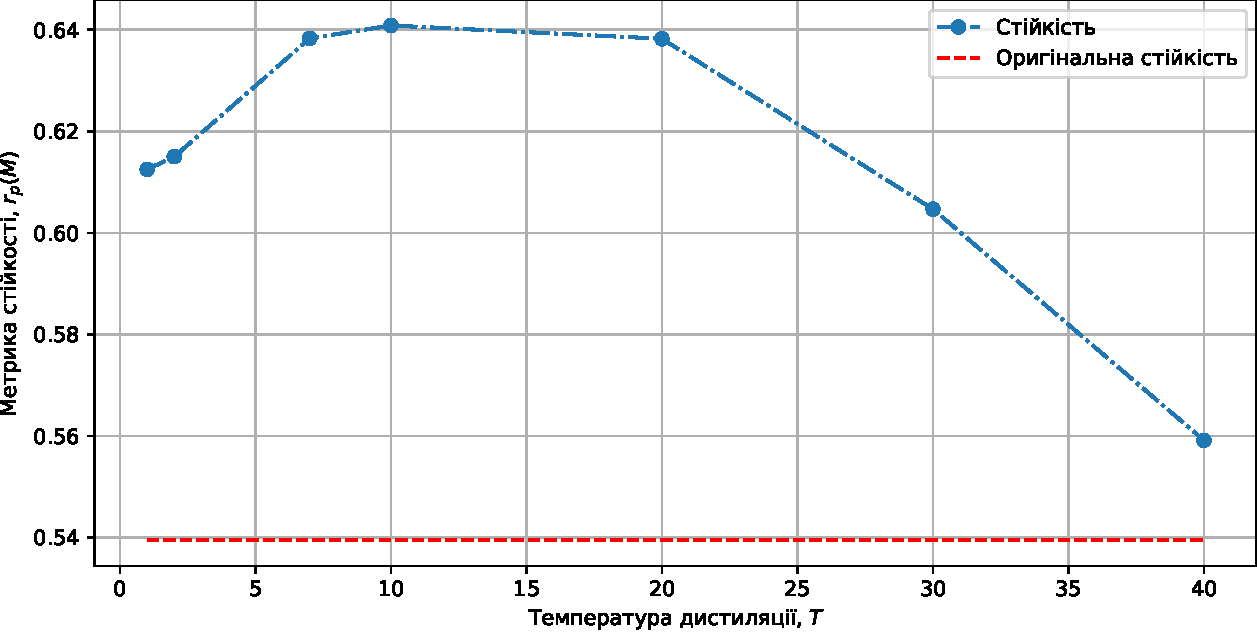
\includegraphics[width=0.8\textwidth]{../images/robustness.pdf}
			
			%\caption{Область $D$}
			%\label{fig:double-connected-region}
		\end{figure}
	
		Ключові зауваження і спостереження
	\end{frame}

	\begin{frame}
		\frametitle{Аналіз точності передбачень}
		\begin{center}
			\begin{tabular}{|c|c|c|c|c|}
				\hline
				\tabboxc{1.3cm}{$T$}
				& \tabboxc{2.3cm}{Точність на $X_{train}$}
				& \tabboxc{2.3cm}{Точність на $X_{test}$}
				& \tabboxc{1.3cm}{$r_p(M)$}
				& \tabboxc{1.3cm}{Приріст стійкості}
				\\ \hline
				
				2
				& 92\%
				& 92\%
				& 0.615
				& 14\%
				\\ \hline
				
				7
				& 90\%
				& 89\%
				& 0.638
				& 18.3\%
				\\ \hline
				
				10
				& 88\%
				& 87\%
				& 0.641
				& 18.8\%
				\\ \hline
				
				20
				& 78\%
				& 77\%
				& 0.639
				& 18.5\%
				\\ \hline
			\end{tabular}
		\end{center}
		Ключові зауваження і спостереження
	\end{frame}

	\begin{frame}

		\begin{figure}[h]
			\centering
			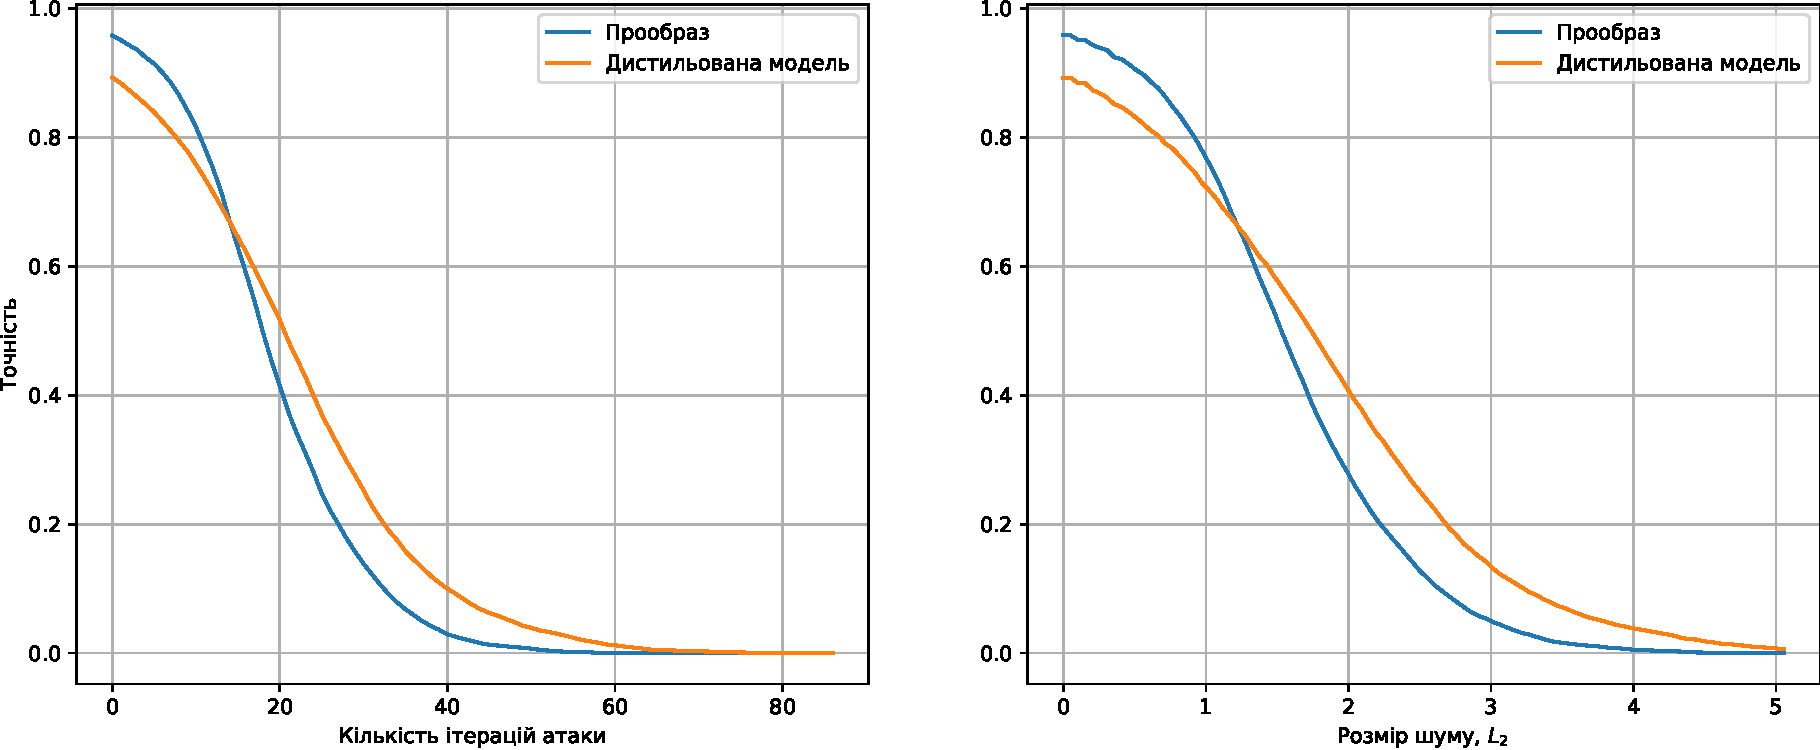
\includegraphics[width=0.8\textwidth]{../images/distAllT7.pdf}
			
			%\caption{Область $D$}
			%\label{fig:double-connected-region}
		\end{figure}
	
	    Ключові зауваження і спостереження
	\end{frame}

	
	%------------------------------------------------
	
	
	%------------------------------------------------
	\section{Висновки}
	%------------------------------------------------
	\begin{frame}
		\frametitle{Висновки}
		
		\begin{itemize}
			\item Стратегії захисту можна розділити на типи
			
			
			\item
		\end{itemize}
		Наш вклад в роботу.
	\end{frame}
		
\section*{Література}
\begin{frame}
	\thispagestyle{empty}
	\frametitle{Література}
	\begin{thebibliography}{99}
		

		\bibitem[1]{defencive-distillation}
		\textit{Nicolas Papernot, Patrick McDaniel, Xi Wu Somesh Jha,Ananthram Swami} /
		Distillation as a Defense to Adversarial Perturbations against Deep Neural Networks /
		arXiv preprint arXiv:1511.04508 (2016)
		
		\bibitem[2]{pixeldp}
		\textit{Mathias Lecuyer, Vaggelis Atlidakis, Roxana Geambasu, Daniel Hsu, Suman Jana} /
		Certified Robustness to Adversarial Examples with Differential Privacy/
		arXiv preprint arXiv:1802.03471 (2019)
		
		\bibitem[3]{analysis-of-robustness}
		\textit{Alhussein Fawzi, Omar Fawzi, Pascal Frossard} /
		Analysis of classifiers' robustness to adversarial perturbations /
		arXiv preprint arXiv:1502.02590 (2016)
		
		\bibitem[4]{my-work}
		\textit{Богдан Бугрій} /
		Атаки на глибокі нейронні мережі /
		Львів (2020)
		
		
	\end{thebibliography}
\end{frame}

\end{document} 